%%%%%%%%%%%%%%%%%%%%
%
% $Beschreibung: Allgemeine Beschreibung der IDE Software $
% $Autor: Hanneken $
% $Datum: 13.05.2024 $
% $Pfad: DemonstratorSchrittmotor/DeveloperDoc/Contents/de/SoftwarebeschreibungIDE.tex $
% $Version: 4 $
%
%
%%%%%%%%%%%%%%%%%%%

\chapter{Beschreibung der Software IDE}

\section{Installation der Arduino IDE}

Die Programmierung von Mikrocontrollern, wie dem verwendeten Arduino Nano 33 BLE Sense Lite, erfolgt unter Verwendung der Software Arduino IDE in der Version 2.3.2.  
Als Alternative kann auch die Entwicklungsumgebung Qt verwendet werden, welche die Programmierung in der Programmiersprache C++ ermöglicht.
Vorteil der Arduino IDE besteht in ihren Funktionen, welche das Einbinden der Software auf dem Mikrocontroller vereinfachen.
Die Software Arduino IDE kann über die offizielle Webseite von Arduino bezogen werden, welche unter der folgenden URL erreichbar ist: \url{www.arduino.cc/software} erreichbar ist. Auf dieser Plattform stehen diverse Versionen, für unterschiedliche Betriebssysteme, wie Windows, Linux und Mac OS X, sowie in verschiedenen Dateiformaten, zur Auswahl bereit \cite{ArdIDE.2024}. Die Installation der Anwendung erfolgt durch die Ausführung der heruntergeladenen Datei sowie die Befolgung der Installationsanweisungen. Im Anschluss ist eine korrekte Konfiguration des verwendeten Entwicklungsboards sowie die Installation entsprechender Bibliotheken erforderlich.

\section{Beschreibung der Entwicklungsumgebung}

Nach dem Start der installierten Anwendung öffnet sich die Hauptoberfläche, erkennbar in Abbildung \ref{HauptoeberflIDE}

\begin{figure}[H]
	\begin{center}
		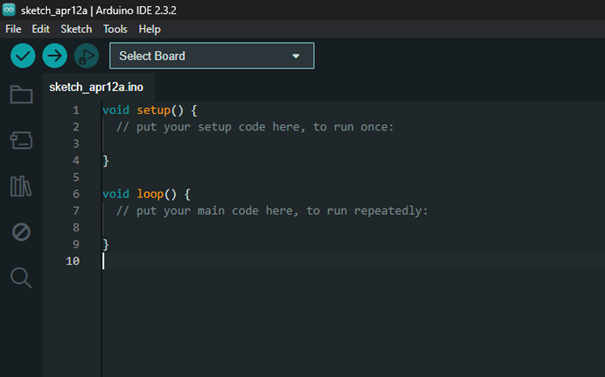
\includegraphics[width=\textwidth]{Images/IDE/HauptoberflaecheIDE.png} 
		\caption{Hauptoberfläche in der Arduino IDE (Eigenaufnahme)} \label{HauptoeberflIDE}
	\end{center}
\end{figure}

Die Hauptoberfläche ist mit einer eine Menüleiste ausgestattet, die verschiedene Menüs wie \textit{Datei}, \textit{Bearbeiten} und \textit{Sketch} enthält. Diese Menüs ermöglichen das Bearbeiten und Öffnen von Sketches, also Programmen in der IDE, das Kompilieren und Hochladen von Code sowie das Verwalten von Bibliotheken. Zudem ist in der Menüleiste ein Hilfe-Menü integriert, das bei Fragen und Problemen Unterstützung bietet. 
Die Symbolleiste auf der linken Seite der Hauptoberfläche bietet Schaltflächen für häufig genutzte Funktionen wie das Verwalten von Sketches, Boards und Bibliotheken.
Im Zentrum der Hauptoberfläche befindet sich ein Code-Editor, welcher die Bearbeitung der Sketches ermöglicht. Nach dem ersten Kompilieren eines Sketches erscheint direkt darunter ein Ausgabefenster, welches den Kompilierungs- und Hochladeprozess sowie eventuelle Fehler während der Kompilierung anzeigt. Dadurch können Probleme im Code schnell identifiziert werden.

\section{Erste Schritte in der Entwicklungsumgebung}

\subsection{Auswahl des Mikrocontrollers}

In der Entwicklungsumgebung können  Sketche geöffnet und geschrieben werden. Um den Sketch kompilieren zu können, ist es erforderlich das korrekte Board auszuwählen.
Dafür muss zunächst das entsprechende Board installiert werden. 
Dies erfolgt über den \textit{Boards-Manager}, erkennbar in Abbildung \ref{Boardsmanager}.
 
\begin{figure}[H]
	\begin{center}
		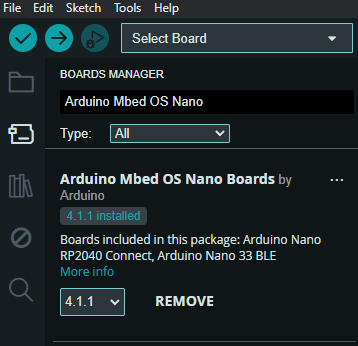
\includegraphics[width=\textwidth]{Images/IDE/Boardsmanager} 
		\caption{Installation des Boards (Eigenaufnahme)} \label{Boardsmanager}
	\end{center}
\end{figure}

Im \textit{Boards Manager} steht die Datei Arduino Mbed OS Nano in der aktuellen Version 4.1.1 zum heruntergeladen und installieren bereit. Im Anschluss kann unter \textit{Select Board} das Board Arduino BLE Sense 33 ausgewählt werden \cite{ArdIDE.2024b}.
Alternativ kann das Board über ein USB-Kabel angeschlossen werden. Unter\textit{ Select Board} wird bereits das korrekte Board und der entsprechende COM, also in diesem Fall der USB-Port, angeboten. Nach der Auswahl sind die Installationsanweisungen zu befolgen, um das Board zu installieren.

\subsection{Bibliotheken einbinden}

Von Arduino gibt es bereits viele offiziell unterstützte Bibliotheken. Um diese in einem Sketch nutzen zu können, ist zunächst eine Installation erforderlich.
Dazu kann über den \textit{Library Manager} die benötigte Bibliothek heruntergeladen und installiert werden, erkennbar in Abbildung \ref{Librarymanager}. Die Suchfunktion hilft dabei, die korrekte Bibliothek zu finden \cite{ArdIDE.2024c}.

\begin{figure}[H]
	\begin{center}
		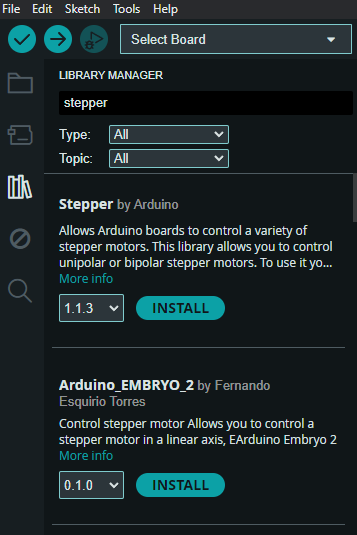
\includegraphics[width=\textwidth]{Images/IDE/Librarymanager} 
		\caption{Herunterladen von Bibliotheken (Eigenaufnahme)} \label{Librarymanager}
	\end{center}
\end{figure}

Nachdem die Bibliothek installiert wurde, kann sie im header in den Sketch eingebunden werden.
Bei Verwendung von Bibliotheken, die nicht im \textit{Library Manager} zu finden sind, besteht die Möglichkeit diese über \textit{Sketch->Include Libraries->Add .ZIP Library…} einzubinden.

\section{Programmierung}
Bei einem neuen Sketch sind bereits die Funktionen \textit{void setup()} und \textit{void loop()} hinterlegt.

\subsection{header}
Im \textit{header} werden die erforderlichen Bibliotheken hinterlegt und initialisiert. Gleichzeitig können hier auch Adressen von Peripheriegeräten hinterlegt und erste wichtige Variablen definiert werden.

\subsection{setup()}
Die \textit{void setup()}-Funktion wird bei jedem Neustart oder Reset einmal ausgeführt \cite{ArdIDE.2024d}.
In diesem Beispiel wird die serielle Kommunikation gestartet, aber auch verwendete Pins initialisiert und zugewiesen.

\subsection{loop()}
In der \textit{void loop()}-Funktion findet der größte Teil des Programms statt. Der Inhalt dieser Funktion wird dauerhaft wiederholt, bis entweder kein Strom mehr an dem Arduino anliegt, oder der Reset-Knopf gedrückt wird, wodurch zunächst erst die \textit{void setup()}-Funktion wieder gestartet wird \cite{ArdIDE.2024e}.

\section{Erster Programmtest}
Um die Funktionalität eines Systems zu testen, wird in der Regel zunächst ein simples Programm oder eine grundlegende Funktion getestet.
In diesem Fall kann hier über \textit{Datei -> Beispiele -> 01.Basics -> Blink} ein Sketch geöffnet werden, in dem die auf dem Arduino Nano 33 BLE Sense Lite aufgebrachte LED in einem fest gelegten Takt blinkt. Auf diese Weise kann die korrekte Auswahl des Boards und die Übertragung des Sketches auf den Mikrocontroller getestet werden.
\ref{Code:Blink}

\begin{code}
	\begin{lstlisting}[language=c++]
void setup() {
	pinMode(LED_BUILTIN, OUTPUT);
}
void loop() {
	digitalWrite(LED_BUILTIN, HIGH);
	delay(1000);                     
	digitalWrite(LED_BUILTIN, LOW);  
	delay(1000);                     
}
\end{lstlisting}      

\caption[Blink.py]{Blink.py}\label{Code:Blink}    
\end{code} 

In der \textit{void setup()}-Funktion wird in diesem Beispiel über den Ausdruck \textit{pinMode(LED BUILTIN, OUTPUT)} die auf dem Mikrocontroller verbaute LED in dem Sketch aufgerufen und eingebunden.
In \textit{void loop()} wird durch den Befehl\textit{ digitalWrite()} die LED eingeschaltet, indem eine Spannung an sie angelegt wird. Nach einer kurzen Verzögerung durch den gleichen Befehl wird die LED dann wieder ausgeschaltet, indem die anliegende Spannung gesenkt wird. Die Verzögerung kann mit dem \textit{delay()}-Befehl eingestellt werden, indem der Wert in der Klammer angepasst wird. Dabei wird der Wert in Millisekunden angegeben.
